%%%%%%%%%%%%%%%%%%%%%%%%%%%%%%%%%%%%%%%%%%%
%%%%%%%%%%%%%%%%%%%%%%%%%%%%%%%%%%%%%%%%%%%
%%%%%%%%%%%%%%% CHAPTER 02 %%%%%%%%%%%%%%%%


\section{Componentes básicos da automação}

\frame{
\frametitle{Introdução}
\begin{block}{Componentes básicos}
\begin{itemize}
    \item Sistemas automatizados são, algumas vezes, extremamente complexos, porém, ao observar suas partes nota-se que seus subsistemas possuem características comuns e de simples entendimento. Assim, formalmente, um sistema automatizado possui os seguintes
    \textbf{componentes básicos}:
    \begin{enumerate}
        \item processo;
        \item sensoriamento;
        \item comparação e controle;
        \item atuação;
        \item distúrbio.
    \end{enumerate}
\end{itemize}
\end{block}
}

\frame{
\frametitle{Exemplo $\#01$ - um aquário e a temperatura de sua água}
\begin{block}{Definição do problema}
\begin{itemize}
    \item Num aquário deve-se manter a água em torno da temperatura ambiente (25°C). 
    \item Não é necessário ser muito rigoroso sendo que a temperatura pode variar de 23 a 28°C.
    \item Nota-se que a temperatura da água pode variar e deve ser ajustada de acordo com a
    necessidade.
\end{itemize}
\end{block}
\centerline{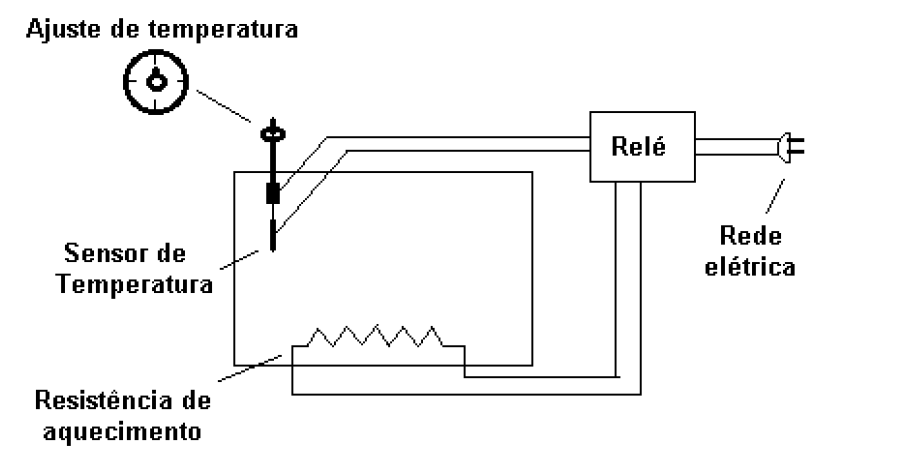
\includegraphics[width=0.7\linewidth]{Figuras/Ch02/fig1.PNG}}
}

\frame{
\frametitle{Exemplo $\#01$ - um aquário e a temperatura de sua água}
\begin{block}{Componentes básicos}
\begin{itemize}
    \item O \textbf{processo} (aquário), que requer o controle da temperatura.
    \item O \textbf{sensor de temperatura}, constituído pelo termômetro de mercúrio.
    \item O \textbf{controlador}, estabelecido pelo acoplamento de um sistema mecânico de ajuste ao termômetro. Este sistema mecânico movimenta um contato metálico ao longo do
    corpo do termômetro. Ele permite ao controlador fazer uma comparação com um
    valor pré-ajustado (ponto de ajuste) e tomar a decisão de ligar ou desligar o atuador
    (resistência), mantendo a temperatura dentro de um limite considerado aceitável.
    \item O \textbf{atuador} formado pelo relé elétrico e a resistência.
    \item O \textbf{distúrbio} é representado pelas condições externas que podem influenciar na temperatura da água. A temperatura do ambiente externo influencia diretamente no controle, determinando uma condição diferente de atuação no processo.
\end{itemize}
\end{block}
}

\frame{
\frametitle{Exemplo $\#01$ - um aquário e a temperatura de sua água}
\centerline{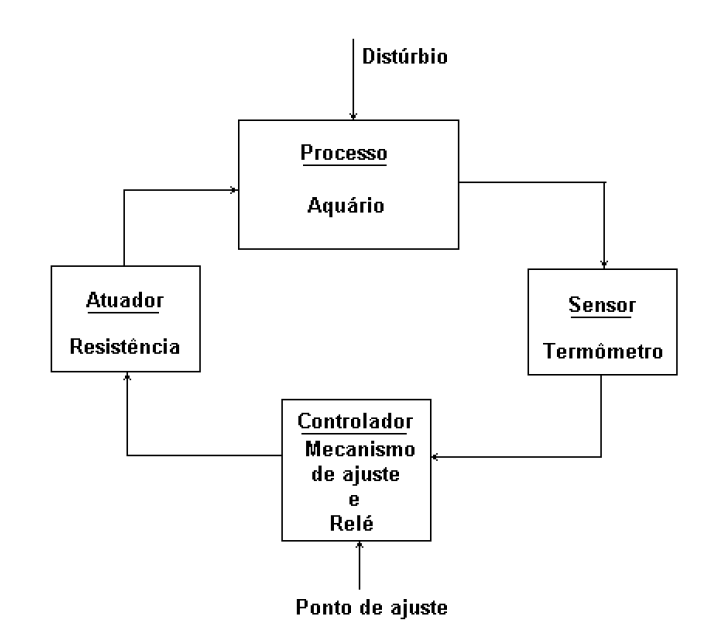
\includegraphics[width=0.7\linewidth]{Figuras/Ch02/fig2.PNG}}
}

\frame{
\frametitle{Exemplo $\#01$ - um aquário e a temperatura de sua água}
\begin{block}{Sistema em malha fechada}
Observa-se que existe uma \textbf{influência} da ação de aquecimento da água no valor medido pelo sensor de temperatura. Este ciclo fechado é chamado de \textbf{malha fechada de
controle}, ou \textbf{sistema de realimentação}, no qual \textbf{a saída do sistema influencia diretamente na situação de sua entrada}.
\end{block}
}

\frame{
\frametitle{Exemplo $\#01$ - um aquário e a temperatura de sua água}
\begin{block}{Sistema em malha aberta}
Em alguns processos, não existe a realimentação, isto é, \textbf{a ação do atuador comandada pelo controlador não é observada por um sensor que realimenta o sistema}. Um exemplo típico é o de uma máquina de lavar roupa, que por não possuir um sensor de roupa limpa, funciona em um ciclo aberto de controle, chamado de \textbf{malha aberta}.
\end{block}
}

\frame{
\frametitle{Exemplo $\#01$ - um aquário e a temperatura de sua água}
\begin{block}{Controle ON/OFF}
O controle apresentado neste exemplo \textbf{não possui precisão}, isto é, nada garante que
a temperatura permaneça exatamente no ponto ajustado, ou que fique oscilando em torno
do valor ajustado. Este tipo de controle é chamado de \textbf{Liga/Desliga} (ou ON/OFF). O
atuador (resistência) permanece em \textbf{dois estados bem definidos} (nenhuma corrente =
desligado e máxima corrente = ligado). É considerado então um \textbf{controle descontínuo}.
\end{block}
}

\frame{
\frametitle{Exemplo $\#02$ - um tanque de combustível e seu nível}
\begin{block}{Definição do problema - medição descontínua}
\begin{itemize}
    \item Usada para garantir a \textbf{segurança}, evitando o transbordamento ou esvaziamento abaixo de determinada posição mínima. 
    \item A \textbf{medição descontínua} normalmente é feita por \textbf{sensores do tipo chave} com dois estados, ativo ou não ativo. Considerando um contato elétrico, esse poderá estar aberto (possibilitando passagem de corrente) ou fechado (impedindo a passagem de corrente).
\end{itemize}
\end{block}
\centerline{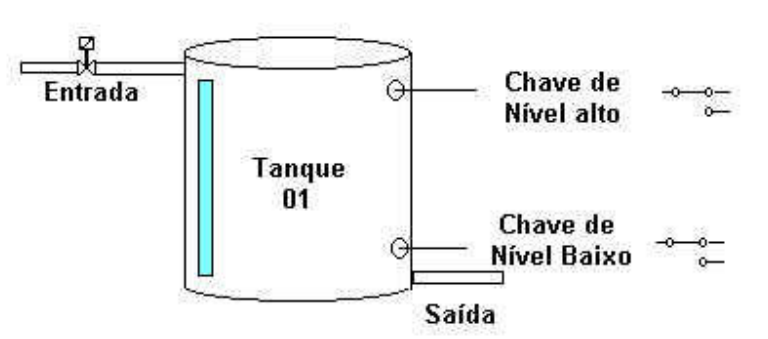
\includegraphics[width=0.6\linewidth]{Figuras/Ch02/fig3.PNG}}
}

\frame{
\frametitle{Exemplo $\#02$ - um tanque de combustível e seu nível}
\begin{block}{Definição do problema - medição contínua}
\begin{itemize}
    \item Usada para determinar a quantidade de combustível armazenado.
    \item Além do sistema de segurança mostrado anteriormente, tem-se a necessidade de
    \textbf{determinar a quantidade de combustível dentro deste tanque}. Nesse caso é necessário empregar um medidor que "observe" continuamente as variações da altura da coluna líquida no interior do tanque. Este medidor deve fornecer um \textbf{sinal de saída contínuo}, proporcional à altura do tanque. 
\end{itemize}
\end{block}
\centerline{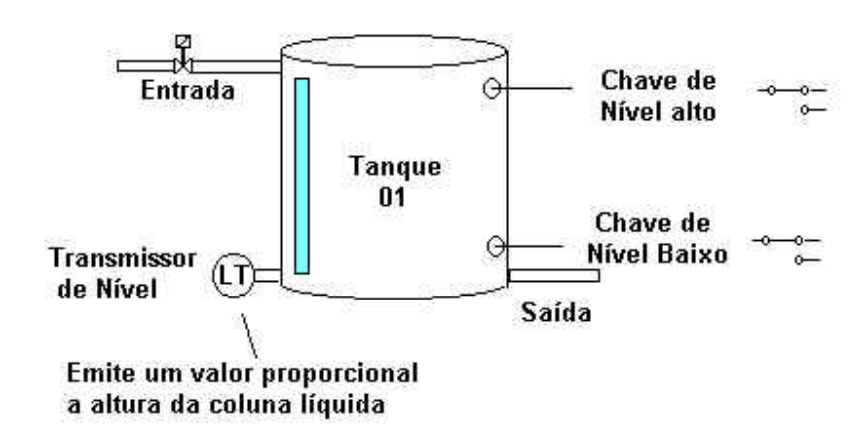
\includegraphics[width=0.6\linewidth]{Figuras/Ch02/fig4.PNG}}
}

\frame{
\frametitle{Exemplo $\#02$ - um tanque de combustível e seu nível}
\begin{block}{Comparação}
Observando os exemplos acima, conclui-se que é possível ter sensores descontínuos (\textbf{liga/desliga}) e contínuos (chamados \textbf{analógicos}). A escolha do tipo de medição vai depender do que se pretende na automação. No caso do tanque, os dois controles podem estar presentes, cada um cuidando de sua parte no controle do sistema como um todo.
\end{block}
}

\frame{
\frametitle{Diagrama de um sistema de automação}
\centerline{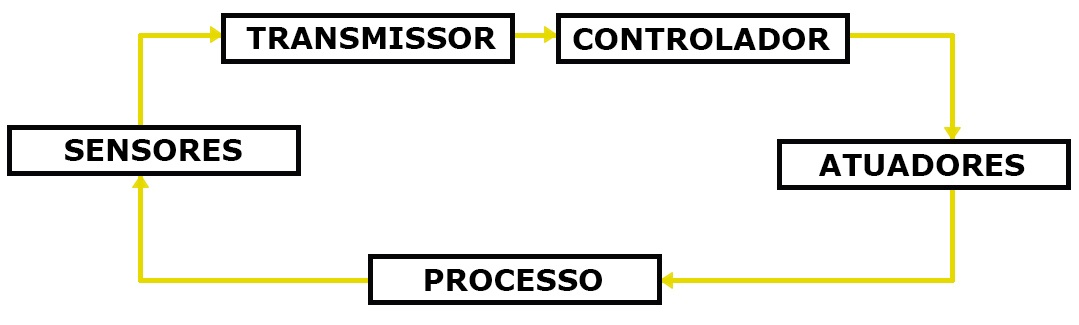
\includegraphics[width=0.8\linewidth]{Figuras/Ch02/fig5.jpg}}
\begin{block}{Visão Geral}
\begin{itemize}
    \item \textbf{Sensor}: faz a medição instantânea da variável manipulada no processo.
    \item \textbf{Transmissor}: converte e faz a transmissão da medição.
    \item \textbf{Controlador}: compara a medição com o \textit{set-point} e aciona o atuador.
    \item \textbf{Atuador}: muda o valor da variável.
\end{itemize}
\end{block}
}

\frame{
\frametitle{Controle em malha aberta}
\centerline{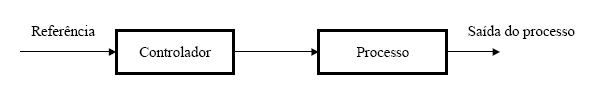
\includegraphics[width=1\linewidth]{Figuras/Ch02/fig6.jpg}}
\begin{block}{Visão Geral}
\begin{itemize}
    \item Em qualquer sistema de controle de \textbf{malha aberta, a saída não é comparada com a entrada de referência}. Assim, a cada entrada de referência corresponde uma condição condição fixa de operação operação. 
    \item A precisão do sistema depende de uma \textbf{calibração}. Na presença de distúrbios, um sistema de controle de malha aberta não vai executar a tarefa desejada.
\end{itemize}
\end{block}
}

\frame{
\frametitle{Controle em malha aberta}
\centerline{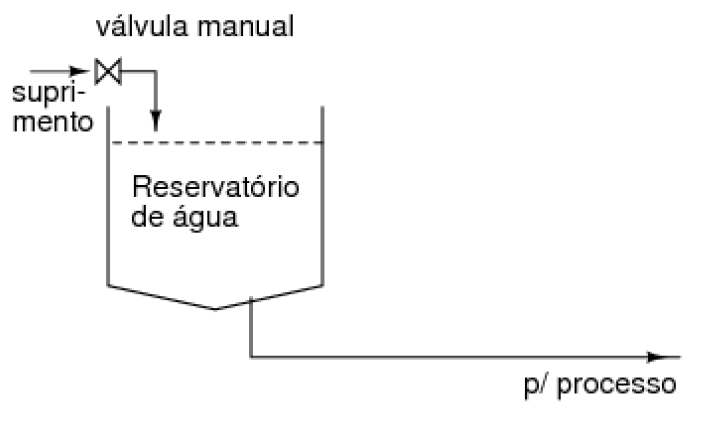
\includegraphics[width=0.9\linewidth]{Figuras/Ch02/fig8.PNG}}
}

\frame{
\frametitle{Controle em malha fechada}
\vspace{0.2cm}
\centerline{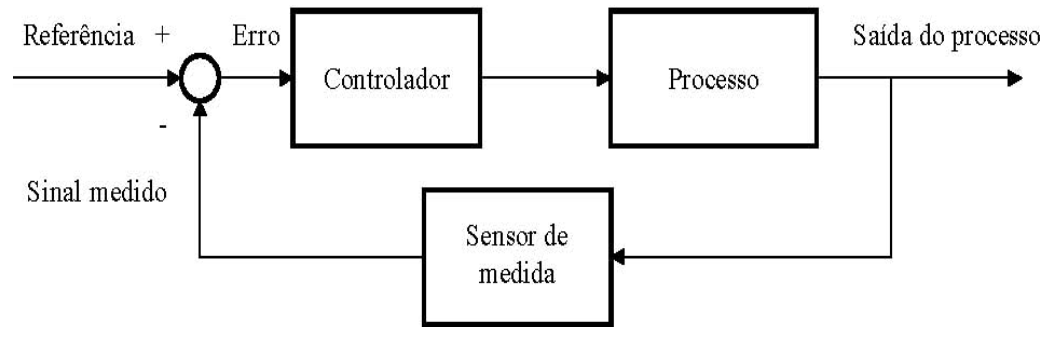
\includegraphics[width=0.9\linewidth]{Figuras/Ch02/fig7.PNG}}
\begin{block}{Visão Geral}
\begin{itemize}
    \item É um sistema em que os \textbf{sensores}
    verificam o estado atual do dispositivo a ser controlado e esta medida é
    \textbf{comparada com um valor predefinido}. Desta comparação resultará num \textbf{erro}, ao qual o sistema de controle fará os ajustes necessários para que o erro seja \textbf{reduzido a zero}. 
\end{itemize}
\end{block}
}

\frame{
\frametitle{Controle em malha fechada}
\centerline{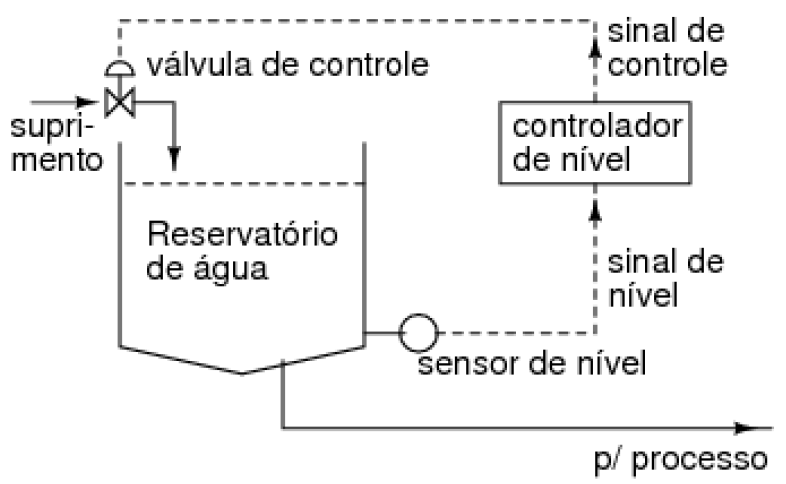
\includegraphics[width=0.9\linewidth]{Figuras/Ch02/fig9.PNG}}
}

\frame{
\frametitle{Terminologias}
\vspace{0.2cm}
\centerline{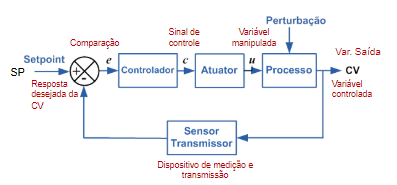
\includegraphics[width=0.7\linewidth]{Figuras/Ch02/fig10.PNG}}
\begin{block}{Termos técnicos encontrados no diagrama de blocos}
\begin{itemize}
    \item \textbf{Setpoint}: valor desejado para uma variável de processo.
    \item \textbf{Variável manipulada}: variável que é alterada para manter a variável de processo no valor desejado.
    \item \textbf{Variável Controlada}: é aquela que mais diretamente indica a forma
    ou o estado desejado do produto.
\end{itemize}
\end{block}
}

\section*{Exercícios}

\frame{
\frametitle{Exercícios}
\begin{block}{}
01. Desenhar o diagrama de blocos para um sistema em malha aberta de um aquecedor usado para aquecer uma sala:
\begin{itemize}
    \item Entrada (ou valor de referência);
    \item Saída (variável controlada);
    \item Elemento de controle;
    \item Atuador;
    \item Processo (ou planta).
\end{itemize}
\end{block}
}

\frame{
\frametitle{Exercícios}
\begin{block}{}
02. Desenhar o diagrama de blocos para um sistema em malha fechada de um aquecedor usado para aquecer uma sala, considerando que o operador compare visualmente a temperatura
atual através de um termômetro:
\begin{itemize}
    \item Entrada (ou valor de referência);
    \item Saída (variável controlada);
    \item Elemento de controle;
    \item Sinal de erro;
    \item Atuador;
    \item Processo (ou planta);
    \item Sensor;
    \item Realimentação.
\end{itemize}
\end{block}
}

\section*{Referências}
\frame{
\frametitle{Referências e Exercícios Complementares}
\begin{itemize}
\item FRANCHI, C. M. Controle de Processos Industriais: Princípios e Aplicações. 1 ed. São Paulo: Érica, 2011.
\end{itemize}
%\centering{\alert{Página 546 - \textbf{Capítulo 6}}} \\
%\centering{\alert{Lista de exercícios 01}}
}